\documentclass{article}
\usepackage[utf8]{inputenc}
\usepackage{float}

\title{\Large{Assignment 1 - Designing Campus LAN Network}}
\author{Tarun Mohandas (2018201008)}
\date{ }

\usepackage{natbib}
\usepackage{graphicx}

\begin{document}

\maketitle

\section{Objective}
To design a Local Area Network for IIIT-Hyderabad campus

\section{Devices Used}
\begin{center}
	\begin{tabular}{ c c c }
		
		Layer 2 Switch & Layer 3 Switch &  Gateway \\ 
		 Firewall & Proxy server &  Wireless access point \\  
		 Repeater & Twisted pair cable &  Fibre optic cable 

    
\end{tabular}

\end{center}

\section{Design Specifications and Considerations}

The large campus is divided into subnets based on the departments, considering each department as a subnet. Although the campus can be considered as one local area, it will be beneficial to divide them into subnets for the following reasons.
\begin{itemize}
	\item Configuration of virtual LAN (VLAN) will be easier when layer 3 is also considered.
	\item It provides flexibility for the campus to grow and expand. More departments can be accommodated into the network.
\end{itemize}
Each subnet consists of one or more LANs. We will discuss IP addressing scheme for the subnets later.

\subsection{LAN Topology}
The LAN in our design, is a combination of star and tree topology. Layer 2 switches are used to do switching between the devices. If the LAN covers a large area and many devices (like hostels), a tree topology is used to combine various switches together. The following diagram shows the aforementioned topology.
\begin{figure}[htb]
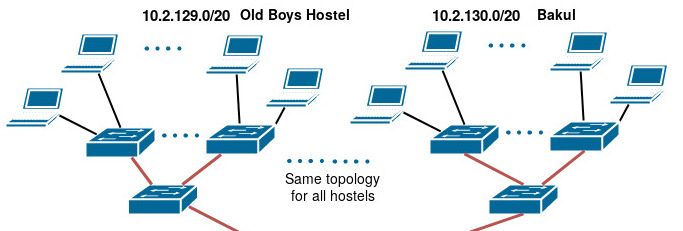
\includegraphics[width=15cm,height=5cm]{hostel.jpg}
\end{figure}
\subsection{LAN Devices}
\subsubsection{Layer 2 Switches}
Layer 2 switches are used in a tree topology as shown above to connect all end devices. Many Layer 2 switches are in-turn connected using start topology to Layer 3 Switch. The Layer 2 Switch must have many \textbf{RJ-45 ports} and a few \textbf{SFP ports}. Generally, switches with SFP ports are costlier than switches with RJ-45 ports. Therefore, the switches we use can have few SFP ports just to connect with other switches. To connect with end devices, we can use RJ-45 ports.
\par
\textbf{SFP (Small Form-factor Pluggable)} ports is in line with 1000BASET (IEEE 802.3ab) standard. The transmission rate of it can reach 1000 Mbps. Built-in SFP ports on switch enable optical or copper links by inserting the corresponding SFP module.

\subsubsection{Layer 3 Switches}
Layer 3 switches are used to divide the campus LAN into subnets for easily configuring VLAN and for managing needs of different departments. The Layer 3 switches we use are \textbf{all SFP port} switches because, at higher levels all departments are connected using fibre optic cable. We use fibre optic cable at higher levels for the following reasons:

\begin{itemize}
	\item Fibre optic cables provide great bandwidth and faster speeds. In a place like a university where there are potentially a large number of people sharing the bandwidth, fibre optic cable provides the necessary support to provide a great bandwidth.
	\item Fibre optic cables can be laid out for larger distances. In a large campus, when data has to be transferred from one place to another in good bandwidth, cables have to be laid out over large distances. Fibre optic cable solves this problem.
\end{itemize}

\subsubsection{Cables}
The end devices are connected to Layer 2 Switches using twisted pair cable (CAT5 or CAT6) using RJ-45 port. We are using twister pair for connecting end devices for the following reasons:
\begin{itemize}
	\item Twister pair cables (copper) are generally cheaper than Fibre optic cable. Students can easily afford twisted pair cables.
	\item RJ45 ports are used to connect twisted pair and switches with RJ45 ports are much cheaper than switches that have huge number of fibre optic ports.
	\item Installation is easier for Twisted pair cables
\end{itemize}

\subsubsection{Wireless Access Points}
Research block, library, and administrative offices are equipped with wireless access points to provide WiFi facility to end devices. The WiFi devices follow the protocol \textbf{802.11 a/b/c}. 20MHz is the most common Wi-Fi bandwidth as most users still opt to use 2.4GHz radios. It supports Gigabit Ethernet. The following diagram shows how devices are connected using WiFi in our network.

\begin{figure}[htb]
	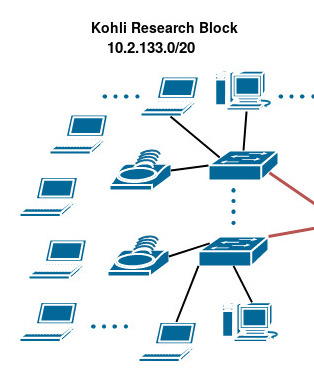
\includegraphics[width=7cm,height=8.5cm]{KRB.jpg}
	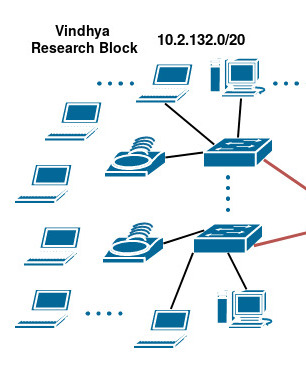
\includegraphics[width=7cm,height=8.5cm]{vindhya.jpg}
\end{figure}

\subsection{Other Devices Used}
\subsubsection{Gateway}
The gateway is used in our network as a device connecting the outer network (typically internet) to the campus LAN. We can configure NAT in this device (discussed in the next part).
\subsubsection{Proxy Server and Firewall}
The proxy server is installed to allow device from outer network access to campus LAN with proper authentication. It can also act central device in configuring VPN involving the campus LAN. Firewall is used to restrict access to ports, sites or particular traffic. This can prove to be very important to college network for various reasons. Firewall can be configured as a separate device or as a software in proxy server or gateway.

\subsubsection{Repeater}
Since this is a large campus and we have relatively few Layer 3 switches, we have to use repeaters to propagate the signal to larger distances. Although the fibre optic cable and its range gives an edge, we can use a repeater to further the signal to its maximum strength. This is an optional device and can be eliminated if using a good fibre optic cable over large distance.

\section{IP Addressing}
Since we are using subnets in our campus LAN, it is important that IP addressing needs to be configured properly with high flexibility. \textbf{NAT (Network Address Translation)} can be used for portability purposes inside the network.
\par
We use Class A IP addressing for our campus. The public IP address we get is 14.0.0.0/8. Since we use NAT, we can configure the standard NAT addressing: 10.0.0.0/8 internally. Although we can configure $2^{24}$ hosts using this IP, we have to split it into subnets. As of now there are a handful of departments in the campus, some of them being:
\begin{itemize}
	\item Server room
	\item Administration
	\item Academics
	\item Research Block
	\item Library and Workspaces
	\item Hostels
\end{itemize}

The number of departments and size of departments can grow in the future and demand more and larger subnets. For this reason we are going to allocate 12 bits of the IP address to network part and 12 bits to host part. Using this we can configure upto $2^{12}=4096$ subnets and around 4094 usable IP addresses per subnet. So our network ID for each of the above network will be 10.1.0.0/20, 10.2.0.0/20 etc. We can assign each of the above mentioned departments to one of the subnets and save the rest for later. The following is an example of how we can distribute IP addresses.

\begin{center}
	\begin{tabular}{ |c|c| }
		\hline
		\textbf{Department} & \textbf{Network ID} \\ 
		\hline
		Server Room & 10.1.0.0/20 \\  
		\hline
		Administration Department & 10.2.0.0/20 \\
		\hline
		Himalaya Block & 10.3.0.0/20 \\
		\hline
		Academics Department & 10.4.0.0/20 \\
		\hline
		Nilgiri & 10.5.0.0/20 \\
		\hline
		KCIS & 10.6.0.0/20 \\
		\hline
		Library and Workspaces & 10.7.0.0/20 \\
		\hline
		Vindhya Block & 10.8.0.0/20 \\
		\hline
		Hostels & 10.8.0.0/20, 10.9.0.0/20...\\
		\hline
	\end{tabular}
\end{center}
\section{Protocols Involved}
\begin{itemize}
	\item 802.3y - 100BASE-T2 100 Mbit/s over voice-grade twisted pair 
	\item 802.3z - 1000BASE-X Gbps Ethernet over Fiber-Optic at 1 Gbpss
	\item 802.3ab - 1000BASE-T Gbps Ethernet over twisted pair at 1 Gbps
	\item 802.11a/b/c - Wireless MAC
	\item IPv4 - Internet Protocol Addressing
\end{itemize}
\section{Network Architecture Diagram (Next page)}
\pagebreak
\begin{figure}[htb]
	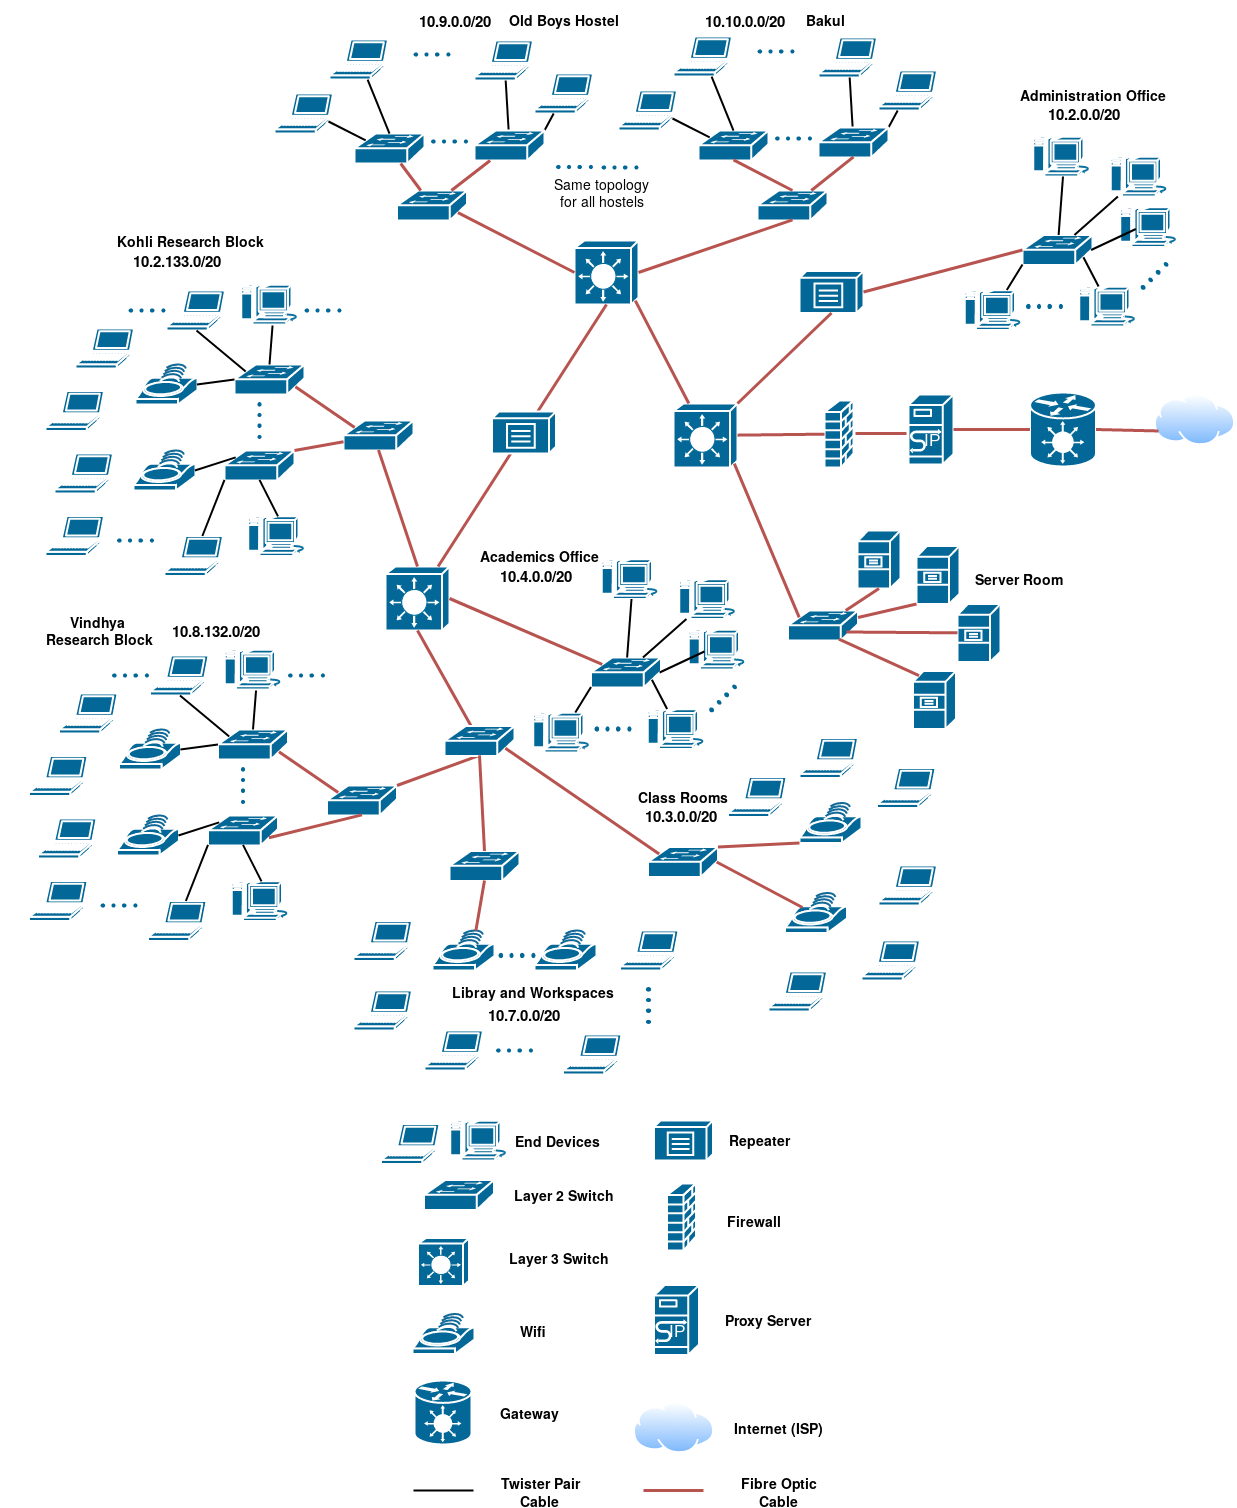
\includegraphics[width=16.5cm,height=23cm]{CampusLan_Final.png}
\end{figure}

\end{document}


